% !TeX root = ../main.tex

% ===================== 緒論 ===================== %
\section{緒論}

% ------------------- 中文測試 ------------------- %
\subsection{研究想法與動機}
隨著第三代合作夥伴計劃（3rd Generation Partnership Project，即 3GPP，是一個國際認可的通訊標準制定組織）第五代行動通訊技術延伸標準（5G-Advanced, 3GPP Release 18）的演進與全球商轉，行動資料流量正迎來前所未有的爆發式增長。為應對增強型行動寬頻（eMBB）帶來的超高資料速率、大規模物聯網（Massive IoT）連接，以及關鍵通訊的嚴苛需求，未來網路的容量將面臨巨大挑戰。

根據 Nokia 於 2016 年發布之 5G 網路能源效率白皮書預測，至 2030 年，全球無線數據流量將可能高達 2010 年的一萬倍 \cite{nokia2016_energy}。伴隨龐大網路容量而來的，是急遽攀升的能源消耗與電信營運商嚴峻的營運成本（Operating Expenditure, OPEX）壓力。該報告明確指出，在成熟的電信市場中，純粹的電力消耗（Electricity）通常佔據了整體網路 OPEX 的 15\%；而在開發中市場，此電力開銷比例更可能高達 30\%，如圖 \ref{fig:network_opex} 所示 \cite{nokia2016_energy}。更關鍵的是，在整個行動網路的總體能源消耗結構中，無線接取網路中的基地台（Base Stations, BS）在總體能源消耗中佔據了高達 80\% \cite{nokia2016_energy}。這項驚人的工業界數據直接表明，基地台正是導致網路營運成本居高不下與碳排放失控的頭號元凶。因此，如何實現數據流量增長與基地台能源消耗的徹底脫鉤，已成為下一代行動網路實現綠色通訊（Green Communications）迫在眉睫的終極願景。

\begin{figure}[htbp]
    \centering
    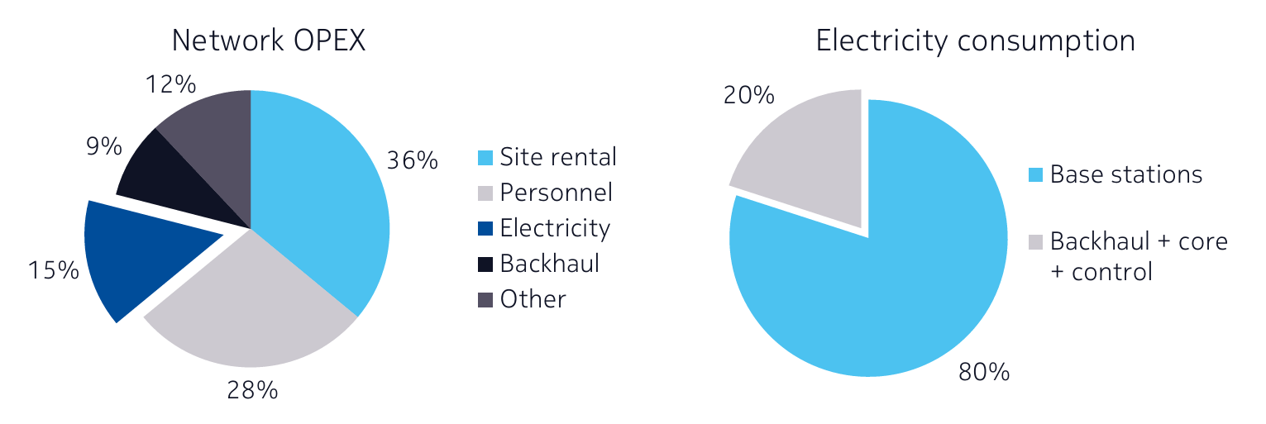
\includegraphics[width=0.9\textwidth]{figures/OPEX開銷圖.png}
    \caption{行動網路營運成本（OPEX）中能源消耗開銷佔比圖（引自 \cite{nokia2016_energy}）}
    \label{fig:network_opex}
\end{figure}

然而，在追求網路容量的同時，真實蜂巢式網路卻面臨著流量在時間維度上顯著起伏的天然挑戰。如歐盟無線網路節能計畫（EARTH Project）之經典文獻 \cite{auer2011_energy} 所定義之每日流量變動模型與圖 \ref{fig:diurnal_traffic} 所示，行動網路流量在一天 24 小時之內存在著顯著的「潮汐效應（Tidal Effect）」——在日間辦公時段與夜間黃金時間，流量會迎來劇烈的尖峰；然而在凌晨至清晨的深夜時段，網路負載則會跌落至極低的谷底。
\begin{figure}[t]
    \centering
    % ⚠️ 注意：這裡將圖片重新命名為 diurnal_traffic.pdf 向量圖格式以確保清晰度
    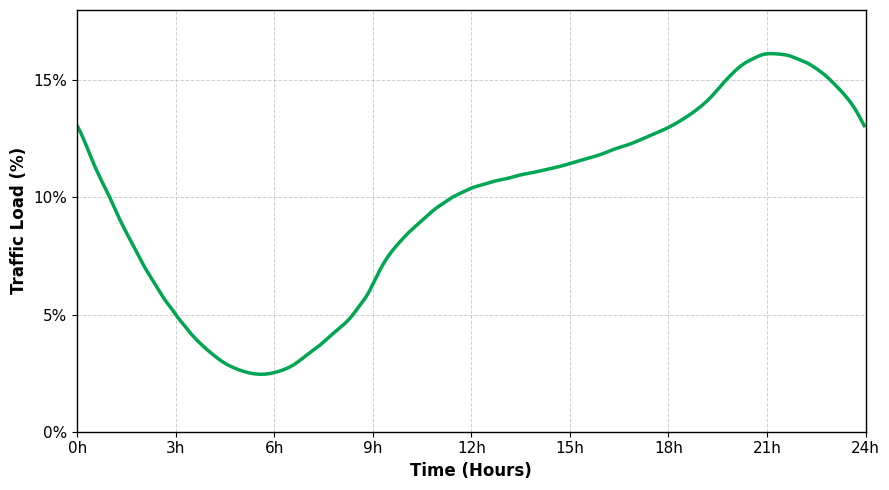
\includegraphics[width=0.75\textwidth]{figures/日網路流量分布.png}
    \caption{真實網路環境中 24 小時流量示意圖（引自 \cite{auer2011_energy}）}
    \label{fig:diurnal_traffic}
\end{figure}
令人遺憾的是，儘管深夜負載極低，傳統基地台的能源消耗曲線在一天中卻顯得極為平坦。探究其根本原
因，在於傳統機制缺乏即時的硬體資源調適能力。在深夜時段，即便實際的使用者資料傳輸量趨近於零，
基地台仍被迫將整體的硬體資源維持在緊繃的最高容量配置狀態。這種僵化的硬體配置導致了嚴重的網路
效能過剩（Over-provisioning），引發高額的無效電力開銷，進而造成巨大的能源浪費。

為了解決上述基地台資源過度配置與效能過剩所導致的電力浪費，並建立國際統一的節能技術標準，3GPP
 於 Release 18 正式確立了 TR 38.864 技術報告 \cite{3gpp2023_tr38864}，專門針對新無線電（New
  Radio, NR）系統的網路節能（Network Energy Saving, NES）技術進行標準化研究。該標準評估
  了不同物理資源維度的節能機制與潛能，指出網路節能主要可從以下四大基礎範疇進行資源調配：
\begin{itemize}
    \item \textbf{時域節能（Time Domain NES）}：藉由行動通訊不連續傳輸（DTX）與不連續接
    收（DRX）之特性，在無數據傳輸的符號或時槽空檔期間，將射頻鏈路（RF chains）切換至低功
    耗運作狀態 。此機制透過精確的時域排程，在維持系統同步性的前提下，最大化硬體元件的非活
    躍時間（Inactivity duration），從而有效削減基地台在閒置期間的固定基礎能耗 。  
    \item \textbf{頻域節能（Frequency Domain NES）}：根據細胞
    當前的實時負載動態調配操作
    頻寬（如調配頻寬部分 BWP）或暫時關閉特定的分量載波（Component Carrier），以減少頻域
    射頻處理開銷。
    \item \textbf{功率域節能（Power Domain NES）}：透過靈活的動態功率控制演算法，在保障
    細胞基礎覆蓋率與連線品質的前提下適度降低發射功率，從而節省功耗並降低細胞間的相互干擾。
    \item \textbf{空間域節能（Spatial Domain NES）}：藉由調整基地台的空間傳輸維度，在低
    負載時動態靜默部分天線單元或關閉部分射頻收發埠（TXRU），直接切斷冗餘鏈路的供電，具備極
    高之節能增益。
\end{itemize}

深入剖析 TR 38.864 標準所規範之基地台功耗模型（Power Consumption Model），可以發現基地台
的功耗組成具有顯著的元件不對稱性。除了執行基本連線、協定疊運算與訊號處理等維持基地台運作所
必需的基頻處理元件（Baseband Processing Units）、主供電模組與散熱系統等固定能耗開銷外，
基地台運作時的主要能耗主體實則集中於負責無線訊號收發與射頻放大的無線射頻鏈路（Radio 
Frequency Chains, RF Chains）以及功率放大器（Power Amplifier, PA）上，其能耗通常佔據總
體功耗的 60\% 以上。基於上述硬體層面之功耗分析，本研究確立了技術選型之邏輯：鑑於維持系統基
本連線與訊號處理功能之基頻元件具有較高之固定功耗，且其功耗隨負載變化之彈性較低，因此，本研
究將焦點置於能耗佔比最高、且最易因流量負載不均而產生硬體配置冗餘之無線射頻鏈路。透過空間域
適應（Spatial Domain Adaptation, SDA）技術，基地台可依據即時之流量負載需求，動態調整啟
用的天線階數與射頻鏈路數量，此機制在維持細胞基礎覆蓋前提下，能提供較佳之節能彈性，故為本研
究探討之重點技術。

然而，現有的 SDA 調適機制普遍面臨「節能（Energy）」與「佇列延遲（Delay）」之間的兩難權衡。
傳統機制多仰賴靜態時程配置或長期平均負載指標進行天線階數切換，當面對 5G 網路常見之高度動態、
具備突發流量（Burst Traffic）特徵的真實環境時往往反應遲滯。這將導致基地台緩衝佇列急遽累積，
進而引發嚴重的延遲（Latency），嚴重破壞使用者的服務品質（Quality of Service, QoS）。

為突破此一技術瓶頸，本研究引入由隨機網路最佳化權威 M. J. Neely 所提出之李雅普諾夫最佳化
（Lyapunov Optimization）理論 \cite{neely2012_lyapunov}。該理論之核心技術優勢在於：系統
無需預先掌握未來流量之統計分佈特徵，即可透過建構「漂移加懲罰（Drift-Plus-Penalty）」之數學
模型，在嚴格確保系統佇列穩定與延遲上限的前提下，將特定的目標函數（即基地台功耗開銷）最小化。
此理論特性極度契合 5G 基地台在面對不可預測之突發流量時，所必須處理的能耗與佇列延遲之權衡問題。
綜合上述背景與技術發展趨勢，本論文套用李雅普諾夫最佳化演算法，設計一套具備高度流量感知能力之
動態天線調適機制。本研究期望在符合 3GPP TR 38.864 標準規範之系統架構下，透過嚴謹之跨層系統
級模擬（System-Level Simulation），驗證所提演算法能即時且動態地於「節能增益」與「佇列延遲」
之間取得最佳化平衡，實現高效之新世代綠色通訊網路。




%\zhlipsum[name=xiangyu]

% ------------------- 英文測試 ------------------- %
\subsection{研究問題}

基於上述 5G-Advanced 網路節能之發展趨勢，以及現有空間域適應（Spatial Domain Adaptation, SDA）技術在實際佈建上之侷限性，本論文旨在透過跨層最佳化理論，解決基地台在高度動態且隨機之流量環境下，難以兼顧「極致節能」與「嚴格服務品質（Quality of Service, QoS）」之技術痛點。為達成此目標，本研究將深入探討以下三個核心技術議題，並以此作為整體系統設計與演算法開發之主軸：

\begin{enumerate}
    \item \textbf{跨層級（MAC-PHY）動態天線決策模型之建立：}\\
    在 3GPP TR 38.864 文件中所定義之複雜基地台功耗模型下 \cite{3gpp2023_tr38864}，基地台的整體輸入功耗深受啟用天線與射頻鏈路（Radio Frequency Chains, RF Chains）數量之影響。然而，傳統天線數量決策機制多僅依賴單一實體層（Physical Layer, PHY）的開路思維進行調控，忽略了天線降維對媒體存取控制層（Medium Access Control, MAC）封包排程與佇列累積之連鎖反應。為此，本研究旨在設計一套創新之李雅普諾夫最佳化（Lyapunov Optimization）作為決策引擎。該模型必須在無需預知未來流量統計特性之嚴苛條件下，精準捕捉 MAC 層佇列延遲（Queue Delay）狀態與 PHY 層硬體動態功耗間的耦合關係，進而建構一套具備跨層感知能力之閉環（Closed-loop）控制框架。    

    \item \textbf{突發流量下乒乓效應之抑制與動態權重調適：}\\
    傳統的李雅普諾夫演算法雖能處理效能權衡問題，但其嚴重依賴靜態配置之控制權重參數（$V$ 值）。當面對 5G 真實網路中極端且瞬息萬變之突發流量（Burst Traffic）時，設定固定的 $V$ 值往往導致系統反應過於遲緩或過度敏感。針對此一缺陷，本研究將改良傳統數學框架，設計一套具備「流量感知」能力之動態 $V$ 值自適應機制。更關鍵的是，為確保演算法在實務系統中之可行性，本研究將探討如何於系統底層引入時間滯後（Timer-based Hold-time）與狀態鎖定等工程容錯設計，以有效抑制因天線頻繁收放所引發之「乒乓效應（Ping-Pong Effect）」，來徹底杜絕佇列延遲發散之風險。
    
    \item \textbf{系統級模擬環境下之效能驗證與權衡分析：}\\
    為驗證所提演算法之商業落地價值，純粹之理論推導已不敷需求。本研究將於符合 3GPP 國際通訊標準之大型時分雙工（Time Division Duplex, TDD）系統級模擬器（System-Level Simulator, SLS）中，進行 C++ 底層模組之改寫與演算法實作。透過導入真實衰雜訊道模型、複雜之多用戶排程邏輯以及動態流量生成器，本研究將精確量化該演算法為網路整體帶來之節能增益（Network Energy Saving Gain）。同時，本研究亦將深入剖析並驗證所提機制在追求極致能效時，其與使用者體驗吞吐量（User-perceived Throughput）及 95 百分位尾部延遲（Tail Latency）之間實際的權衡邊界（Trade-off Boundaries）。
\end{enumerate}

透過逐一解析並克服上述三大研究議題，本論文期望能突破傳統天線調適機制之瓶頸，為下一代綠色行動通訊網路，提供一套兼具嚴謹數學理論基礎與實務工程落地價值之動態資源調度解決方案。




\subsection{研究貢獻與論文架構}

針對上述研究議題，本論文旨在將嚴謹之數學最佳化理論與 5G 實務網路部署進行整合。本研究之具體貢獻可歸納為以下三點：
\begin{enumerate}
    \item \textbf{建立跨層級之空間域適應（SDA）最佳化框架：} 本研究成功將李雅普諾夫最佳化（Lyapunov Optimization）理論導入 5G 基地台天線調適機制中，實現了涵蓋媒體存取控制層（Medium Access Control, MAC）封包佇列延遲與實體層（Physical Layer, PHY）整體系統功耗之跨層級（Cross-layer）聯合最佳化。
    \item \textbf{開發增強型通道狀態資訊（Enhanced CSI）評估機制：} 為實現精確的 SDA 天線決策，本研究於 C++ 系統層級模擬器（SLS）中開發了 Enhanced CSI 探測模組。該機制能即時量測多組 SDA 天線配置下之通道品質資訊，提供決策引擎準確之傳輸速率預測依據，從而確保動態降維操作下之連結可靠度，解決了單一固定天線配置無法彈性適應通道變化之瓶頸。
    \item \textbf{創新流量感知動態權重調適與容錯設計：} 針對傳統李雅普諾夫演算法之權重參數（$V$ 值）靜態限制，本研究設計了具備「流量感知」能力之動態 $V$ 值自適應機制，並引入時間滯後（Timer-based Hold-time）與狀態鎖定等工程防呆設計，成功消除突發流量下之天線乒乓效應（Ping-Pong Effect），實現了網路能效（ESG）與服務品質（QoS）之最佳化權衡。
\end{enumerate}

為完整呈現上述研究過程與成果，本論文之章節架構安排如下：

\textbf{第二章 文獻探討}：探討 5G-Advanced 網路節能（NES）之技術演進，回顧 SDA 技術現況，並論述李雅普諾夫最佳化之理論基礎與本研究之技術定位。

\textbf{第三章 系統模型與研究方法}：詳細定義網路場景、基地台功耗模型與 MAC 層佇列動態模型。同時，闡述本研究實作之 Enhanced CSI 量測機制，說明其如何為 SDA 決策引擎提供多組配置下的通道效能資訊，並進行李雅普諾夫決策引擎之數學推導。

\textbf{第四章 系統模擬與效能分析}：說明符合 3GPP 國際標準之 C++ 系統級模擬環境建置。透過大規模動態流量場景，驗證 Enhanced CSI 與動態李雅普諾夫決策引擎之協作效能，深入剖析節能增益、吞吐量與尾部延遲（Tail Latency）間的權衡關係。

\textbf{第五章 結論與未來展望}：總結本論文之核心貢獻，並針對未來 6G 網路下更複雜之多維度聯合節能技術，提出後續延伸研究方向。